\chapter{基于并行的大规模知识图谱表示学习框架}
\label{cha:framework}

\section{简介}

% 正如我们之前提到

% % Knowledge graphs (KGs) are playing an important role in many applications such as question answering and web search. These applications require embeddings of entities and relations in KGs for efficient compution. A variety of effective methods have been proposed to embed KGs into continuous low-dimensional spaces. The implementations of these methods have been verified on small KGs, but not fast enough to embed large-scale KGs. To alleviate this issue, we present OpenKE, an efficient implementation framework for knowledge graph embedding via multi- threading training and some algorithmic design optimizations for acceleration. The evaluation results show that our frame- work can significantly improve embedding efficiency with comparable performance. We also provide embeddings of the exist- ing large-scale KGs, including Freebase and Wikidata, learned by our framework, which can be directly used for relevant ap- plications. Our toolkits and embeddings are released on our website 1.


% People construct various large-scale knowledge graphs (KGs) to organize structural knowledge about the world, such as WordNet \cite{miller1995wordnet}, Freebase \cite{bollacker2008freebase} and Wikidata \cite{vrandevcic2014wikidata}. These typical KGs are often organized in the format of multiple relational directed graphs. Nodes in KGs are corresponding to entities, and edges in KGs are corresponding to relations between these entities. Hence, the facts in KGs are usually recorded as a set of relational triples ($h$, $r$, $t$) with $h$ and $t$ indicating \emph{head} and \emph{tail} entities and $r$ indicating the relation between $h$ and $t$, e.g., (\emph{Mark Twain}, \texttt{PlaceOfBirth}, \emph{Florida}). After a long time of constructing and collating, information in the existing KGs is structural and clear, which can be used to help various applications get better performance, such as question answering and web search.

% \begin{figure*}[t]
% \centering
% \includegraphics[width=0.9\linewidth]{3.jpg}
% \caption{The overall framework of OpenKE}
% \label{fig:joinglearning}
% \end{figure*}

% To incorporate KGs into these applications, we need to embed entities and relations as input. Meanwhile, though most existing KGs are large, they are far from completion, which is also partially solved by embedding KGs recently. Thus, a variety of representative approaches have been proposed to encode entities and relations into a continuous low-dimensional space based on the network structure of KGs, such as graph-based models \cite{lao2010relational,lao2011random}, tensor-based models \cite{socher2013reasoning, nickel2016holographic} and translating models \cite{bordes2013translating,ji2015knowledge,ji2016knowledge}. TransE \cite{bordes2013translating} is a typical translating models, which regards the relation $r$ in each fact ($h$, $r$, $t$) as a translation from $h$ to $t$ within the low-dimensional space, i.e., $\textbf{h} + \textbf{r} = \textbf{t}$. Because TransE is an effective and efficient method that possesses good performance, it has many extensions, including TransH \cite{wang2014transh}, TransR \cite{lin2015learning}, TransD \cite{ji2015knowledge}, etc. 

% Although these translating models have achieved great results on small benchmark datasets, the existing implementations of these models are often single-thread and very time-consuming for training, which can not work well for embedding large-scale KGs. To learn large-scale knowledge graph embeddings, we propose some optimization methods. The optimization methods of our works are threefold. First, we design a unified framework to accelerate TransE and its extensions. The framework separates the overall KG into several parts and adopts these models for multi-threading training. We also propose the offset-based negative sampling to replace origin negative sampling algorithms in this framework. The new sampling mechanism can merge arithmetic operations for acceleration. Second, for some specific models, we also implement them by TensorFlow \cite{Abadi2016TensorFlow} based on our framework to build a convenient platform to run models on GPUs \footnote{https://github.com/thunlp/TensorFlow-TransX}. Third, besides the toolkits, we also provide pre-trained embeddings of large-scale KGs by this framework. The embeddings can be used directly for other works.

% We name our works as OpenKE. The experiment results show that OpenKE achieves great speedup ratio without harming the accuracy and efficient enough to learn large-scale KGs.





% \section{相关工作}

% 知识表示学习的代表模型主要包括距离模型、
% 双线性模型、神经张量模型、矩阵分解模型、翻译 模型等。

  
%     \subsection{早期的表示模型}
  
%     \subsection{基于张量的表示模型}
%       \subsubsection{RESACL}
%       \subsubsection{NTN}
%       \subsubsection{Hole}
%     \subsection{基于平移的表示模型}
%       \subsubsection{TransE}
%       \subsubsection{TransH}
%       \subsubsection{TransR}
%       \subsubsection{TransD}



\section{算法框架}

在这一章节内容里,我们主要介绍我们设计出的开放式知识图谱嵌入结构 OpenKE。内容包括 OpenKE 在并行模式下实现的大规模知识图谱表示学习框架,以及已有的知识图谱模型在框架 OpenKE 下进行实现和融合的具体方式和实施细节。整体的模型骨架我们可以在图\ref{fig:openke}中看到。在整个框架中,底层操作和上层模型是独立的,上层模型可以自由选择和适配,而底层结构则是我们进行了大量优化之后的并行架构。进一步讲,这样一个解耦合的框架使得一个新提出的模型也可以在无需过多关注底层的情况下得到高效实现,具有高自由度和高效率的特点,这些都将在之后的内容里详细铺开。当然,在介绍具体细节之前,我们先引入一些符号体系和重要概念。


\begin{figure*}[h]
\centering
\includegraphics[width=1.0\linewidth]{figures/ch2/3.jpg}
\caption{基于并行的大规模知识图谱表示学习框架 OpenKE 的结构示意图}
\label{fig:openke}
\end{figure*}

\subsection{符号体系和重要概念}

我们将整个知识图谱定义为一个由实体集、关系集和事实三元组集合共同组成的大集合,即$G = \{E, R, T\}$,这里$E$、$R$和$T$分别表示实体集合、关系集合和事实三元组集合。对于事实三元组集合中的任意事实$(h, r, t) \in T$,这个三元组表明头实体$h \in E$和尾实体$t \in E$之间存在一个逻辑上的关联$r \in R$。由于表示学习会将实体和关系都嵌入到连续空间中去并用对应的向量来表示他们的语义信息,所以对于任意的实体或者关系$h, t \in E$或$r \in R$,我们都用它们的加粗字母$\mathbf{h}, \mathbf{t}, \mathbf{r}$来表示它们的向量,这里的向量也可以称为嵌入、嵌入向量、表示、嵌入表示等。

\subsection{知识图谱表示学习模型}

对于知识图谱表示学习,模型需要做的就是将实体和关系嵌入到连续空间中,从而利用空间向量来表达它们之间存在的语义关联。在这里,我们先以一个统一的数学视角来归纳这些模型方法,从而方便之后在底层上进行统一的实现。然后我们接着给出在具体实现时,以 TransE 为代表的平移模型各自之间的不同之处。

在知识图谱表示学习模型中,通常先定义一个能量函数来衡量事实三元组的合理程度。更准确的说,对于任意一个给定的三元组$(h, r, t)$,模型会为之定义一个能量函数$S(h, r, t)$。如果三元组是合理的,比如$(h, r, t)\in T$,此时的能量函数将返回一个较低的值。相反,如果三元组是不成立的,那么能量函数则会返回一个较高的值。这个函数通常情况下和$h, r, t$在空间上的距离具有相关性,换句话说,存在关联的实体与关系在空间上也是相近的。

对于包括 TransE 及其一系列的拓展模型在内的基于平移的知识图谱表示模型,会定义一个潜在的向量表示$r_{ht}$来具象化头实体和尾实体$(h, t)$之间的潜在关系。这些模型之所以叫做基于平移的表示模型,是因为它们都遵循``关系在空间中是实体向量间的平移变换''这个基本假设。在这个假设下,如果三元组成立,那么会有潜在向量$\textbf{r}_{ht}$和显式的关系向量$\textbf{r}$在空间上极为接近。换句话说,我们获取头实体和尾实体之间关系的过程,就是一个寻找与潜在关系向量$\textbf{r}_{ht}$在空间上最近的关系向量的过程,由此我们将能量函数定义为两者的空间距离:
\begin{align}
\label{eq:energy functions}
S(h, r, t) & = \lVert \textbf{r} -  \textbf{r}_{ht} \rVert_{L1/L2}
\end{align}
这里,能量函数$S(h, r, t)$可以用L1距离衡量,也可以用L2距离衡量。在能量函数的基础上,我们可以进一步得到一个基于边界值优化的损失函数来作为我们的训练目标,并有如下公式:
\begin{align}
\label{eq:loss}
& \mathcal{L}(G) = \sum_{(h,r,t) \in T} \sum_{(h',r,t')\in T'} \big[ \gamma + S(h,r,t) - S(h', r, t') \big]_{+}
\end{align}
这里,$[x]_{+}$是这样一个函数,如果$x$是正数的话,那么返回值就是$x$,反之返回值为$0$。$\gamma > 0$是一个边界值,用来约束损失函数的训练。$S(h, r, t)$是正例三元组的能量函数得分,而$S(h', r, t')$是负例三元组的能量函数得分,$T'$是负例三元组的集合。这样的损失函数表明,我们希望正确的三元组和负例三元组的能量函数尽可能拉开差距,但又不能使训练过拟合,所以选定一个边界值并在其范围内进行最大化区分度的训练,这也是这些模型一脉相承的设计思路。而对于负例三元组集合$T'$有:
\begin{equation}
T' = \{(h',r,t)\}  \cup \{(h,r,t')\},
\end{equation}
负例三元组集合是通过将正例三元组$(h, r, t) \in T$中的实体替换成其他实体集合中的实体$h', t' \in E$来构造的。

在有了上述统一的损失函数和训练方法之后,我们可以基于几乎相同的边界值训练模式在我们的框架中来实现 TransE \cite{bordes2013translating}、TransH \cite{wang2014transh}、TransR \cite{lin2015learning}、TransD \cite{ji2015knowledge} 等诸多模型。这些模型主要的区别在于它们潜在关系向量$\textbf{r}_{ht}$计算方式的不同,其余部分和上述模型归纳一致。对于这些模型之间的区别和变化,我们接下来将详细罗列并介绍。

\textbf{TransE.} 在 TransE 中,对于每个三元组$(h, r, t)$,我们定义出以下的潜在关系向量$\textbf{r}_{ht}$和能量函数$S(h,r,t)$:
\begin{align}
&\textbf{r}_{ht} = \textbf{t} - \textbf{h},  \\\nonumber
&S(h, r, t) = \lVert \textbf{h} + \textbf{r} - \textbf{t} \rVert_{L1/L2}
\end{align}
由此可以看出,所谓的平移假设,实际上就是希望空间上满足$\mathbf{h}_r + \mathbf{r} \approx \mathbf{t}_r$。

\textbf{TransH.} 在 TransH 中,对于每个给定的实体,其在不同的关系环境下具有不同的嵌入表示。对于每个三元组$(h, r, t)$,我们定义出以下的潜在关系向量$\textbf{r}_{ht}$和能量函数$S(h,r,t)$:
\begin{align}
&\textbf{h}_r = \textbf{h} - \textbf{w}_r^{\top} \textbf{h} \textbf{w}_r, \\\nonumber
&\textbf{t}_r = \textbf{t} - \textbf{w}_r^{\top} \textbf{t} \textbf{w}_r, \\\nonumber
&\textbf{r}_{ht} = \textbf{t}_r - \textbf{h}_r,  \\\nonumber
&S(h, r, t) = \lVert \textbf{h}_r + \textbf{r} - \textbf{t}_r \rVert_{L1/L2}
\end{align}
这里$\textbf{w}_r$是一个归一化之后的向量,用来作为关系$r$所在平面的法向量。

\textbf{TransR.} 在 TransR 中,实体和关系是在不同的空间中被学习得到的,并且实体之间的平移性质是在关系向量所在的空间中进行的。对于每个三元组$(h, r, t)$,我们定义出以下的潜在关系向量$\textbf{r}_{ht}$和能量函数$S(h,r,t)$:
\begin{align}
& \textbf{h}_r = \textbf{M}_r \textbf{h} , \\\nonumber 
& \textbf{t}_r = \textbf{M}_r \textbf{t} , \\\nonumber
& \textbf{r}_{ht} = \textbf{t}_r - \textbf{h}_r,  \\\nonumber
& S(h, r, t) = \lVert \textbf{h}_r + \textbf{r} - \textbf{t}_r \rVert_{L1/L2}
\end{align}
这里$\textbf{M}_r$是关系$r$的映射矩阵,用来将实体从实体空间映射到关系空间中,以方便平移性质的实现。

\textbf{TransD.} 在 TransD 中,实体和关系同样是在不同的空间中被学习得到的。TransD 和 TransR 是十分相似的,但是其采用了动态的映射矩阵来进行映射。对于每个三元组$(h, r, t)$,我们定义出以下的潜在关系向量$\textbf{r}_{ht}$和能量函数$S(h,r,t)$:
\begin{align}
&\textbf{h}_{r} = \textbf{M}_{rh}\textbf{h}, \\\nonumber
&\textbf{M}_{rh} = \textbf{r}_p\textbf{h}_p^{\top}+\textbf{I}, \\\nonumber
&\textbf{t}_{r} = \textbf{M}_{rt}\textbf{t},  \\\nonumber
&\textbf{M}_{th} = \textbf{r}_p\textbf{t}_p^{\top}+\textbf{I}, \\\nonumber
&\textbf{r}_{ht} = \textbf{t}_r - \textbf{h}_r,  \\\nonumber
& S(h, r, t) = \lVert \textbf{h}_r + \textbf{r} - \textbf{t}_r \rVert_{L1/L2}
\end{align}
这里$\textbf{r}_p$和$\textbf{h}_p, \textbf{t}_p$都是用来生成映射矩阵$\textbf{M}_{rh}$和$\textbf{M}_{rt}$的映射向量。通过这样的映射方式,矩阵运算变为了向量运算,在保持了一定映射性质的情况下加快了整体训练速度。


\begin{algorithm}[t]
  \caption{并行学习伪代码}
  \label{algo1}
  \begin{algorithmic}[1]
        \Require 

        实体和关系集合$E, R$,

        训练三元组$T = \{(h, r, t)\}$,

        边界值$\gamma$,嵌入空间维度,

        训练轮数$epoches$,线程数$threads$,一批次训练数据量$batches$。
        \State \textbf{初始化} 

        $\textbf{e} \leftarrow $ uniform$ ( -\frac{6}{\sqrt{k}}, \frac{6}{\sqrt{k}}) $,对于任意$e \in E$;

        $\textbf{r} \leftarrow $ uniform$ ( -\frac{6}{\sqrt{k}}, \frac{6}{\sqrt{k}}) $,对于任意$r \in R$。

    \State \textbf{初始化}

    其他参数,比如:

    TransH 的$\textbf{w}_r$;

    TransR 的$\textbf{M}_r$;

    TransD 的$\textbf{r}_p, \textbf{h}_p, \textbf{t}_p$。
    
    \For {$i \leftarrow $ $1$ to $epoches$}
      \State 在每一个线程中:
      \For {$j \leftarrow $ $1$ to $batches/threads$}
      \State 采样正例 $(h, r, t)$
      \State 采样负例 $(h', r, t')$
      \If{$\gamma + S(h, r, t) - S(h', r, t') \textgreater 0$}
      \State \textbf{更新梯度} $\nabla \big[ \gamma + S(h,r,t) - S(h', r, t') \big]_{+}$
      \EndIf
      \EndFor
      \EndFor
    \State \textbf{返回} 训练得到的实体嵌入和关系嵌入
  \end{algorithmic}
\end{algorithm}

\subsection{并行结构}

在统一了各个知识图谱表示学习模型的形式之后,我们可以发现,这些模型除了上层的能量函数计算方法略有差距外,整体的底层结构,包括采样算法在内都是一致的。所以我们的框架在这些已有模型的底层基础之上,修改了部分结构以便于进行算法加速。其中极为重要的一点就是将知识图谱上的数据划分为若干部分训练三元组集合,并将模型改造成多线程形式来处理每一部分的集合。这样一个并行的学习方法在算法\ref{algo1}中给出了伪代码。

我们的并行学习结构采用的是基于数据并行的多线程机制,并且以此为基础实现了两种梯度更新的策略来训练模型。其中一种方法是通过无锁策略实现的,即所有的线程共享同一块内存空间,优化损失函数时可以实时地将导数反馈到内存中。因为没有加锁,所以在这个策略下,多个线程是可能出现竞争修改同一块内存的。所有线程共享统一的嵌入空间,直接更新嵌入而不进行同步操作,虽然这降低了梯度下降的质量,但整体上的速度提升效果非常明显。另一方面,我们还实现了一个中心同步梯度的方法。对于每个线程,它会计算其自身部分数据的梯度。当所有的线程都计算完毕后,中心会将整体的梯度进行加和,汇总后得到整体的梯度,然后这个结果将会被统一地反馈到实体和关系的嵌入向量或者其他参数上。

值得注意的是,同样的实体对或者实体关系对,可能在同一训练周期内被不同的线程同时计算到,这些重复运算是可以避免的,所以我们也合并了这些算术运算以便进一步加速我们的底层框架。



\begin{algorithm}[t]
  \caption{基于位移的负例采样算法}
  \label{algo2}
  \begin{algorithmic}[1]
      \Ensure 将所有实体$e \in E$映射为连续整数编码$num_e \in \{0, ..., \lVert E \rVert  - 1\}$。
        \Require 

        需要替换的三元组$(h, r, t)$,

        所有和$h, r$匹配的尾实体集合$E_{hr} = \{t|(h,r,t)\in T\}$。

        对于任意实体$e \in E_{hr}$,我们用其整数编码来进行排序,其在$E_{hr}$中的排名为$rank_e \in \{0, ..., \lVert E_{hr} \rVert  - 1\}$。
        \State $p \leftarrow $ rand$(0, \lVert E \rVert - \lVert E_{hr} \rVert)$
        \State $\hat{e} = \mathop{\arg\max}_{e \in E_{hr}} (num_{e}-rank_{e})$,这里需满足 $num_{e}-rank_{e} \leq p$,$num_{e}-rank_{e}$具有偏序关系所以可用二分来解决。
        \State \textbf{返回} 生成的负例三元组$(h, r, t')$,这里$t'$有$num_{t'} = p + rank_{\hat{e}}$
  \end{algorithmic}
\end{algorithm}


\subsection{基于位移的负例采样算法}

对于 TransE 及其一系列的拓展模型,它们的优化过程都是以最小化其基于边界值的损失函数而进行的,即最小化式\ref{eq:loss}。从大量的实践中我们发现,负例三元组的选择对最后的模型效果有着至关重要的影响。在前文介绍的负例三元组生成模式下,负例三元组集合$T'$是通过随机使用$E$中实体替换正例三元组的头尾实体来构建的。由于很多关系并不是一对一的模式,这意味着这套替换机制有可能用另一个正确的实体替换了当前的实体,$T'$中极有可能含有一些$T$中出现过的三元组。举个例子,替换机制将(\emph{美国},\emph{总统},\emph{奥巴马})替换为(\emph{美国},\emph{总统},\emph{克林顿}),两者都是正确的三元组。在实际处理中,如果替换实体之后生成的三元组在$T$中出现,那么这个三元组将不会被用作负例来处理。因此,在原有的负例采样算法中我们会花费大量时间来检验采样出的三元组是否在$T$中出现。为了优化此处的时间复杂度,我们提出了基于位移的负例采样算法来直接生成负例而无需进行任何检验。我们以替换尾实体为例,将该算法伪代码罗列在算法\ref{algo2}中。

在算法操作过程中,对于所有实体,我们用从$0$开始的连续的整数定义它们的整数编码,并且以此排序来使得实体集合具有序列性质,之后我们的各项操作都可以建立在这些整数编码之上。在替换过程中,我们首先随机一个编码。接着,我们采取了这样一个采样思路——如果存在非候选项(即$E_{hr}$中不能用来替换的实体),其整数编码落在随机数的范围内,我们就在随机编码的基础上加对应数量的偏移,从而将所有的非候选项都错开,并得到一个负采样的三元组。直观上讲,这个方法就是将所有的实体排列在一条线上,其中不能替换的实体会将整个直线划分为若干个线段,如果随机落点落在某个线段内则可以直接返回,如果随机落点出现问题落在顶点上的话,我们就将落点偏移使得落点只会在线段之内,这样生成的三元组是一定不会在$T$中出现的。

\section{实验设计与结果分析}

我们选取了知识图谱上的链接预测任务来进行框架性能的评测。在这里,我们一方面会对我们的框架 OpenKE 进行各种性能上的测试,另一方面我们会将结果与一个已经被广泛使用的工具包 KB2E \footnote{https://github.com/thunlp/KB2E}进行对比来体现 OpenKE 的高效性。KB2E 是 Lin 等人\cite{lin2015learning} 在论文发表后开源的工具包,其中实现了 TransE、TransH以及其自身工作 TransR在内的诸多知识图谱表示学习模型。KB2E 因为效果稳定而在很多工作中被使用,并且开源在 Github 上可以直接被获取。

在实验部分,所有的测试都是在$16$GB内存的单机上进行的,处理器为 Intel Core i7-6700K,拥有$4$个核心、$8$个线程,处理器的基本频率为$4.00$GHZ。

\subsection{实验数据集}

在实验中,我们选取了 FB15K 和 WN18 \footnote{https://everest.hds.utc.fr/doku.php?id=en:transe}这两个数据集合来进行测试。数据集合 FB15K 和 WN18 是知识图谱表示学习模型的主要评测基准,并在过去的大量工作中被广泛使用。这两个数据集合都是从公开的大型知识图谱中经过采样得到的子集,其中 FB15K 的内容是从 Freebase 中抽取出的,WN18 的内容是从 WordNet 中抽取出的。我们在表\ref{tab:statistics-of-FB15K}中详细罗列了 FB15K 和 WN18 的整体数据细节。

\begin{table}[htb]
\centering
\caption{FB15K 和 WN18 的数据细节}
\scalebox{1.0}{
\begin{tabular}{|c|c|c|c|c|c|}
\hline
Dataset & Relation & Entity & Train & Valid & Test \\ \hline
FB15K   & 1,345           & 14,951            & 483,142 &50,000 &59,071 \\ \hline
WN18   & 18           & 40,943            & 141,442  &5,000 &5,000 \\ \hline
\end{tabular}}
\label{tab:statistics-of-FB15K}
\end{table}

\subsection{实验与模型参数设置}
为了与之前的模型以及对应论文中公布的实验结果能够合理地进行对比,我们在实验参数的设定上遵循了之前知识图谱表示学习模型通用的办法。经验上,我们选择了边界值$\gamma = 4$来训练 WN18 下的各个模型,而对于 FB15K 我们则用$\gamma = 1$作为训练的边界值。在之前一些工作的实验中,TransE、TransH 以及 TransR 在$50$维上表现明显,TransD 在$100$维度上表现明显,所以我们将 TransE、TransH 以及 TransR 的嵌入向量维度设置为$50$,而将 TransD 的嵌入向量维度设置为$100$。无论是 FB15K 还是 WN18 我们均训练所有的模型$1000$轮以控制拟合的程度相对一致,且一轮训练会将数据划分为$100$批来进行处理。


\subsection{实验评估方式}
在 TransE \cite{bordes2013translating} 被提出时,链接预测就作为重要的评测方式来度量模型的嵌入表达能力。其评测方式为:给定一个头实体和关系的组合$(h, r, ?)$来预测对应的尾实体,或者给定一个尾实体和关系的组合$(?, r ,t)$来预测对应的头实体,预测的依据则是模型根据知识图谱结构学到的嵌入表示。在具体实施细节上,对于任意给定的测试三元组$(h, r, t)$,我们枚举所有的实体来替换头实体$h$以及尾实体$t$,并使用式\ref{eq:energy functions}计算能量得分,之后按照升序排列。根据我们归纳出的模型数学性质,$(h, r, t)$如果成立的话,其得分应当比替换后的三元组得分要低,即$h, t$的隐关系向量$\textbf{r}_{ht}$和$r$的向量在空间上是最接近的。这里我们仍然举个例子来说明,如补全三元组(\emph{?},\emph{著作},\emph{威尼斯商人})时,意味着我们在回答``《威尼斯商人》是谁的著作?''这个问题,这时我们要把所有的实体都尝试一下并给出对应的得分,如果模型合理的话,\emph{莎士比亚}被带入时会得到最优的评分。

和之前提到的相关工作一样,我们使用正确实体能量得分排在前十的比例来衡量预测质量,我们将这个结果称为$10$预测命中率(Hits@10)。因为我们需要的是模型整体的预测效能,并且从实践中来看$1$命中很难做到,也不是很好对模型质量进行细粒度区分,所以过去的模型和我们都选择了$10$预测命中率来进行实验。此外,我们也报告了正确实体的平均排序名次(Mean Rank),这个指标结果一定程度上直观体现了整体向量的学习质量。

我们之前也提到过,一个通过替换实体得到的新三元组很有可能是图谱中存在的正例三元组,该三元组其实不应当被算作是错误而存在。如需补全三元组(\emph{美国}, \emph{总统}, \emph{?})时,意味着我们在回答``美国总统是谁?''。如果三元组本身是(\emph{美国},\emph{总统},\emph{奥巴马}),但将\emph{奥巴马}替换成\emph{华盛顿}后有一个更好的评分,这并不能看作是一个失败的预测,甚至是模型低能的体现,毕竟(\emph{美国},\emph{总统},\emph{华盛顿})也是成立的。所以在替换完实体之后,在排名之前,我们将这些正确的三元组过滤掉,然后进行之前的 Hits@10 和 Mean Rank 的指标评估,这个结果我们称之为``Filter'',而没有经过过滤操作的结果我们称之为``Raw''。

在训练过程中,当替换三元组的实体时,我们遵循 Wang \cite{wang2014transh} 提出的两种方法,即 ``unif'' 和 ``bern''。``bern'' 采用不同概率来替换头尾实体,对于非一对一的关系,我们会对实体可能性较多的部分给予更多的关注和更大的概率来生成负例。而过去一贯等概率替换头或者尾实体的方法被命名为``unif''。使用不同的决策会导致不同的实验结果,对于所有的模型我们同时使用 ``unif'' 和 ``bern'' 两种决策来训练模型,并且在各项指标里选择较优的结果来代表模型的泛化能力。

\subsection{实验结果与分析}

对于涉及到的模型的实验结果,我们直接引用了对应论文里汇报的数据,并且记录为其对应模型名。在我们的框架 OpenKE 下实现的各个模型,其实验结果被命名为模型名加``OpenKE''后缀,比如 TransE(OpenKE)。由于我们会与工具包 KB2E 中实现的模型来进行效率对比,所以我们引入了 KB2E 中的 TransE,命名为 TransE(KB2E)。

所有的实验结果都罗列在表\ref{tab:performance_comparison1}之中。除此以外,我们还报告了在不同的线程设定之下,损失函数的下降曲线,不同模型在不同线程设置下的加速比,这些分别体现在图\ref{fig:loss}和图\ref{fig:speedup}中。



\begin{table*}[h]  
  % footnotesize
  \centering  
  \caption{链接预测的结果}  
  % \fontsize{7}{9}\selectfont  
  \label{tab:performance_comparison1}  
  \scalebox{0.94}{
    \begin{tabular}{|c|c c|c c|c|c c|c c|c|}  
    \hline    
    Data Sets&\multicolumn{5}{c|}{WN18}&\multicolumn{5}{c|}{FB15K}\\\cline{1-11}
    \multirow{2}{*}{Metric}&
    \multicolumn{2}{c|}{Mean Rank}&
    \multicolumn{2}{c|}{Hits@10(\%)}&
    \multirow{2}{*}{time(s)}&
    \multicolumn{2}{c|}{Mean Rank}&
    \multicolumn{2}{c|}{Hits@10(\%)}&
    \multirow{2}{*}{time(s)}
    \cr
    {}&Raw&Filter&Raw&Filter&{}&Raw&Filter&Raw&Filter&{}\cr
    \hline
  
    TransE(KB2E)&251&239&78.9&89.8&1674&210&82&41.9&61.3&3587\cr
    TransE(OpenKE)&273&261&71.5&83.3&12&205&69&43.8&63.5&42\cr
    TransE&263&251&75.4&89.2&-&243&125&34.9&47.1&-\cr\hline      
    TransH(OpenKE)&285&272&79.8&92.5&121&202&67&43.7&63.0&178\cr  
    TransH&318&303&75.4&86.7&-&221&84&42.5&58.5&-\cr\hline         
    TransR(OpenKE)&284&271&81.0&94.6&296&196&73&48.8&69.8&1572\cr
    TransR&232&219&78.3&91.7&-&198&77&48.2&68.7&-\cr\hline      
    TransD(OpenKE)&309&297&78.5&91.9&201&236&95&49.9&75.2&231\cr 
    TransD&224&212&79.6&92.2&-&194&91&53.4&77.3&-\cr\hline   

    \end{tabular}}  
\end{table*}

\begin{figure*}[h]
\small
\begin{minipage}[]{0.5\linewidth}
\centering
\setcaptionwidth{2.8in}
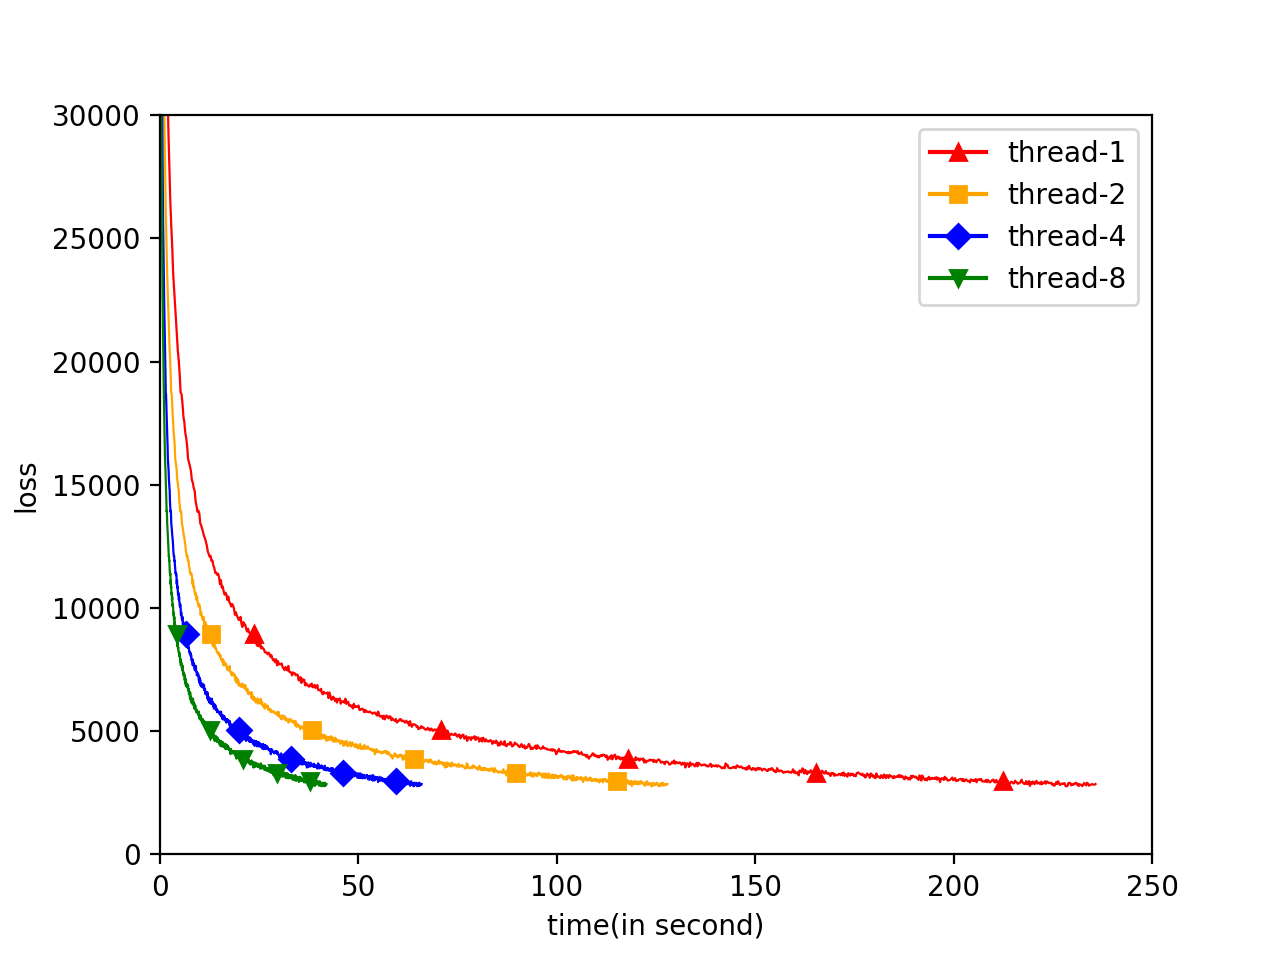
\includegraphics[width=1\linewidth]{figures/ch2/FB15-transE-loss.png}
\caption{在不同线程设定下,TransE 在 FB15K 上的损失函数走向}
\label{fig:loss}
\end{minipage}
\begin{minipage}[]{0.5\linewidth}
\centering
\setcaptionwidth{2.8in}
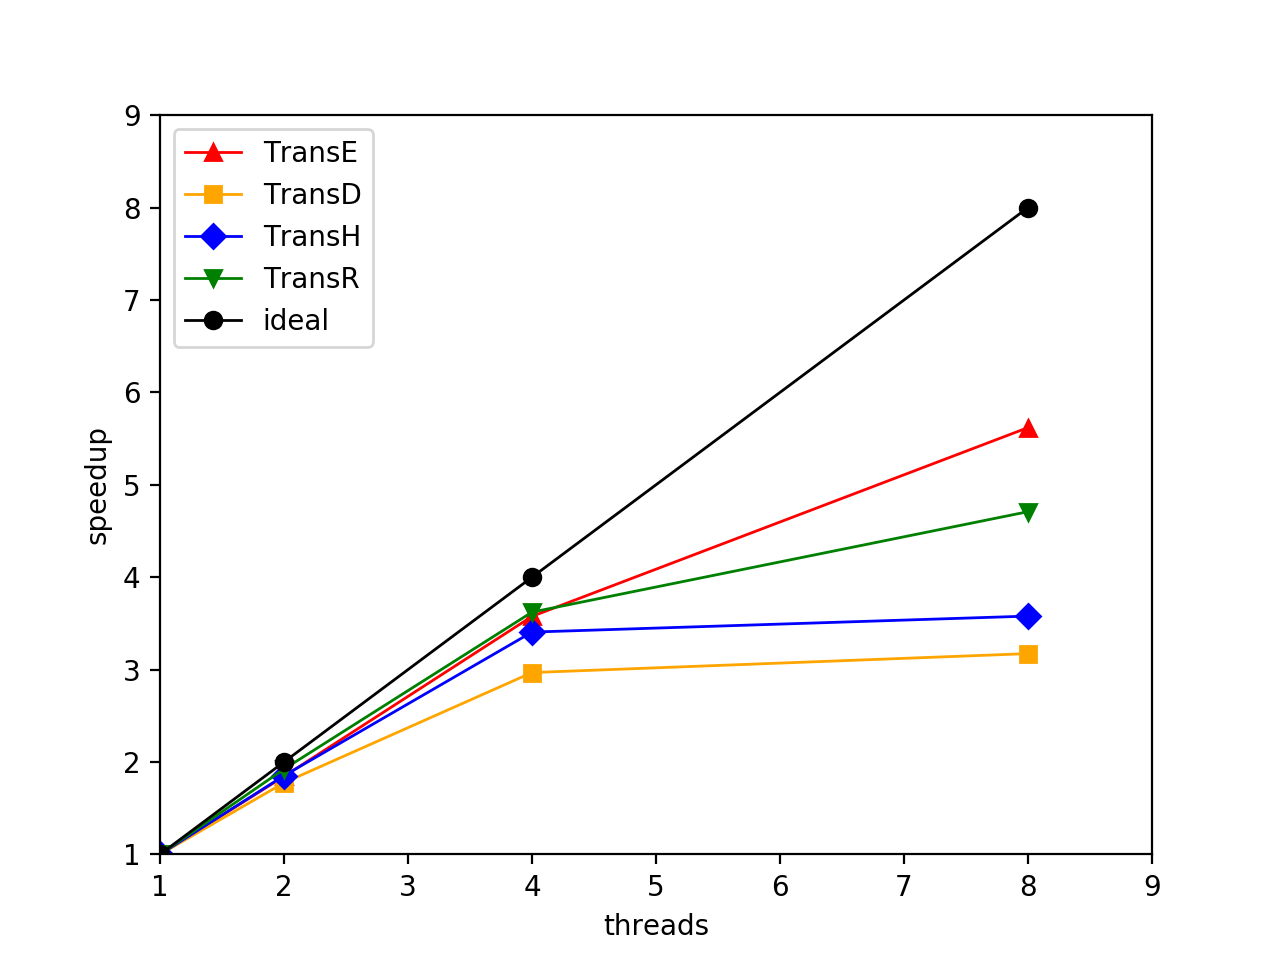
\includegraphics[width=1\linewidth]{figures/ch2/FB15K-transR-speedup.png}
\caption{在不同线程设定下,OpenKE 下不同模型的加速比曲线}
\label{fig:speedup}
\end{minipage}
\end{figure*} 

从这些结果我们可以发现:

(1) KB2E \cite{lin2015learning} 是一个对之前知识图谱表示学习模型非常有效的实现,其评测结果比论文原始结果要高出许多。而和 KB2E 相比,OpenKE 下学到的模型在时间上要短的多,并且效果也非常接近,这意味着 OpenKE 极大的优化了训练速率并且没有影响模型性能。从整体来看,TransE 在 OpenKE 上的实现比其在 KB2E 上的实现加速了85倍。这么大的加速比一方面是因为 KB2E 是一个底层单线程的框架,而我们的 OpenKE 却是基于数据并行的并行框架。但是在$8$线程的处理器上,即使是理想情况,即不计通信同步时间,多线程加速比的极限也不会高于$8$。所以,我们$85$倍的加速除了有多线程的贡献外,另一个重要的因素就是我们基于位移的负例采样算法和底层算术运算合并带来的积极作用。实际上,这些非算法结构上的优化对实际耗时的减少至关重要。


(2) 通过链接预测的结果,可以发现在我们的框架 OpenKE 下训练的模型,基本取得了与原始报告数据非常接近的准确度,并且在其中部分模型上,在 OpenKE 下实现可以获得略高的精度,这些现象和我们的预期是相符合的。因为我们的数据并行机制对在 OpenKE 下实现的模型没有影响,尤其是不会改变这些模型的数学性质,直观上讲我们的框架将一批数据分给若干个线程处理,而每个线程的处理方式和单线程是一致的。与其他模型相比,TransR 需要更多的时间来学习知识图谱的嵌入表示,这主要是 TransR 需要将实体通过映射矩阵投影到关系空间中,而矩阵运算其实是一个计算瓶颈,并且在CPU上很难解决。为了减轻矩阵运算带来的计算瓶颈,我们还在相同底层结构的框架上给出了 GPU 版本的模型实现。因为其模型性质和 CPU 版本是一致的,所以我们只是给出 GPU 版本的链接而不在实验中进行度量,链接附在本章节引言部分处。

(3) 伴随线程数的不断增多,损失函数下降需要的时间以及各模型和单线程相比的加速比都有了变化。从损失函数的下降曲线以及实际加速比曲线可以看到,多线程框架带来的优化以及耗时的下降非常的显著。当线程数小于$4$时,加速比与线程数几乎成正比,也基本接近理想的加速情况。当使用超过$4$个线程时,由于线程调度中的通信和同步,并行能力受到很大影响,加速比的上升速度开始逐渐缓慢甚至保持不变。这其中的影响因素主要来自于我们所采用的处理器。我们的处理器虽然有$8$个线程,却只有$4$个计算核心,这意味着在使用超过$4$个线程时,每个核心将需要负载至少两个的工作线程,线程的切片和通信过频会导致效率下降,所以出现了两个图表后半段加速比停滞的情况。实际上,如果采用更适合并发的处理器,这个停滞的现象将会在更多的线程被启用时才出现,而不是仅仅超过$4$个线程就接近瓶颈,这也启发我们在当前工作的基础上继续采用分布式而非单卡的框架来进行加速。

总的来说,各项评估结果表明,我们的框架成功解决了之前模型实现存在的巨大耗时问题,从而使得这些已经被提出的算法能够真正地对大规模的知识图谱进行表示学习。我们整合了这些模型底层的共通之处,使得新算法可以在不考虑底层繁琐细节的情况下也能得到高效实现。事实上,基于我们 OpenKE 的 TransE 只需耗时$18$个小时就可以训练整个 Wikidata 达$10000$轮左右,并可以获得一个稳定的嵌入表示。我们在引言部分介绍过,wikidata 是一个拥有超过$2500$万实体的巨大知识图谱。这些预先学习好的嵌入表示我们将其公开在网络 \footnote{http://openke.thunlp.org/} 上供直接使用。

\section{本章小结}

对于真正的大规模知识图谱表示学习问题,我们提出了一个有效的训练框架 OpenKE 以便在现有模型基础上进行改进,从而能够解决我们的需求。与此同时,我们也基于该框架提供了已训练完成的大规模知识图谱嵌入向量,使得部分应用可以直接使用而无需再去耗时训练向量。我们的框架采用了基于数据并行机制的并行学习方式,从而能够取得数倍的速度提升。除此以外,我们还提出了基于位移的负例采样算法以及部分基础算术运算合并来进一步加速训练。在实验部分,链接预测上的实验结果表明,在通用的评测数据上我们的底层设计可以帮助现有模型有效地提高效率。而各个模型也在不剧烈影响精度的情况下显著缩短了训练的时间。目前在我们 OpenKE 架构下,部分模型得到了高效复现并且已经能够在真实的大规模知识图谱上进行训练。在未来,我们还将探索并尝试在 OpenKE 的框架下实现更多的知识图表示学习模型。此外,在现有基于多线程的并行学习模式之外,我们还将尝试构建分布式架构来进一步解决规模和时耗问题。在我们的工作中,我们也基于 TensorFlow 来为 OpenKE 实现了一个相对简单的GPU版本,在我们未来的工作中,使用高效的GPU底层框架也是一个十分有意义的方向。
